\section{Metodologia}
\label{sec:metodologia}



\subsection{Exemplos de istas}

\begin{itemize}
\item Esse é um exemplo de lista de tópicos. 
{\color{blue}
\item Lorem ipsum dolor sit amet, consectetur adipiscing elit, sed do eiusmod tempor incididunt.
\item Lorem ipsum dolor sit amet, consectetur adipiscing elit, sed do eiusmod tempor incididunt ut labore et dolore magna aliqua. Ut enim ad minim veniam.
\item Lorem ipsum dolor sit amet, consectetur adipiscing elit, sed do eiusmod tempor incididunt ut labore et dolore magna aliqua. Ut enim ad minim veniam.}
\end{itemize}


\begin{enumerate}%
\item Esse é um exemplo de lista numerada.
{\color{blue}
\item Lorem ipsum dolor sit amet, consectetur adipiscing elit, sed do eiusmod tempor incididunt.
\item Lorem ipsum dolor sit amet, consectetur adipiscing elit, sed do eiusmod tempor incididunt ut labore et dolore magna aliqua. Ut enim ad minim veniam.
\item Lorem ipsum dolor sit amet, consectetur adipiscing elit, sed do eiusmod tempor incididunt ut labore et dolore magna aliqua. Ut enim ad minim veniam.}
\end{enumerate}



\subsection{Exemplos de inclusão de imagens}

Referência de figuras no texto \textbf{Figure \ref{Fig1}} que se expandem em uma única coluna.\textbf{Figure \ref{Fig1}}.


\begin{figure}
\begin{center}
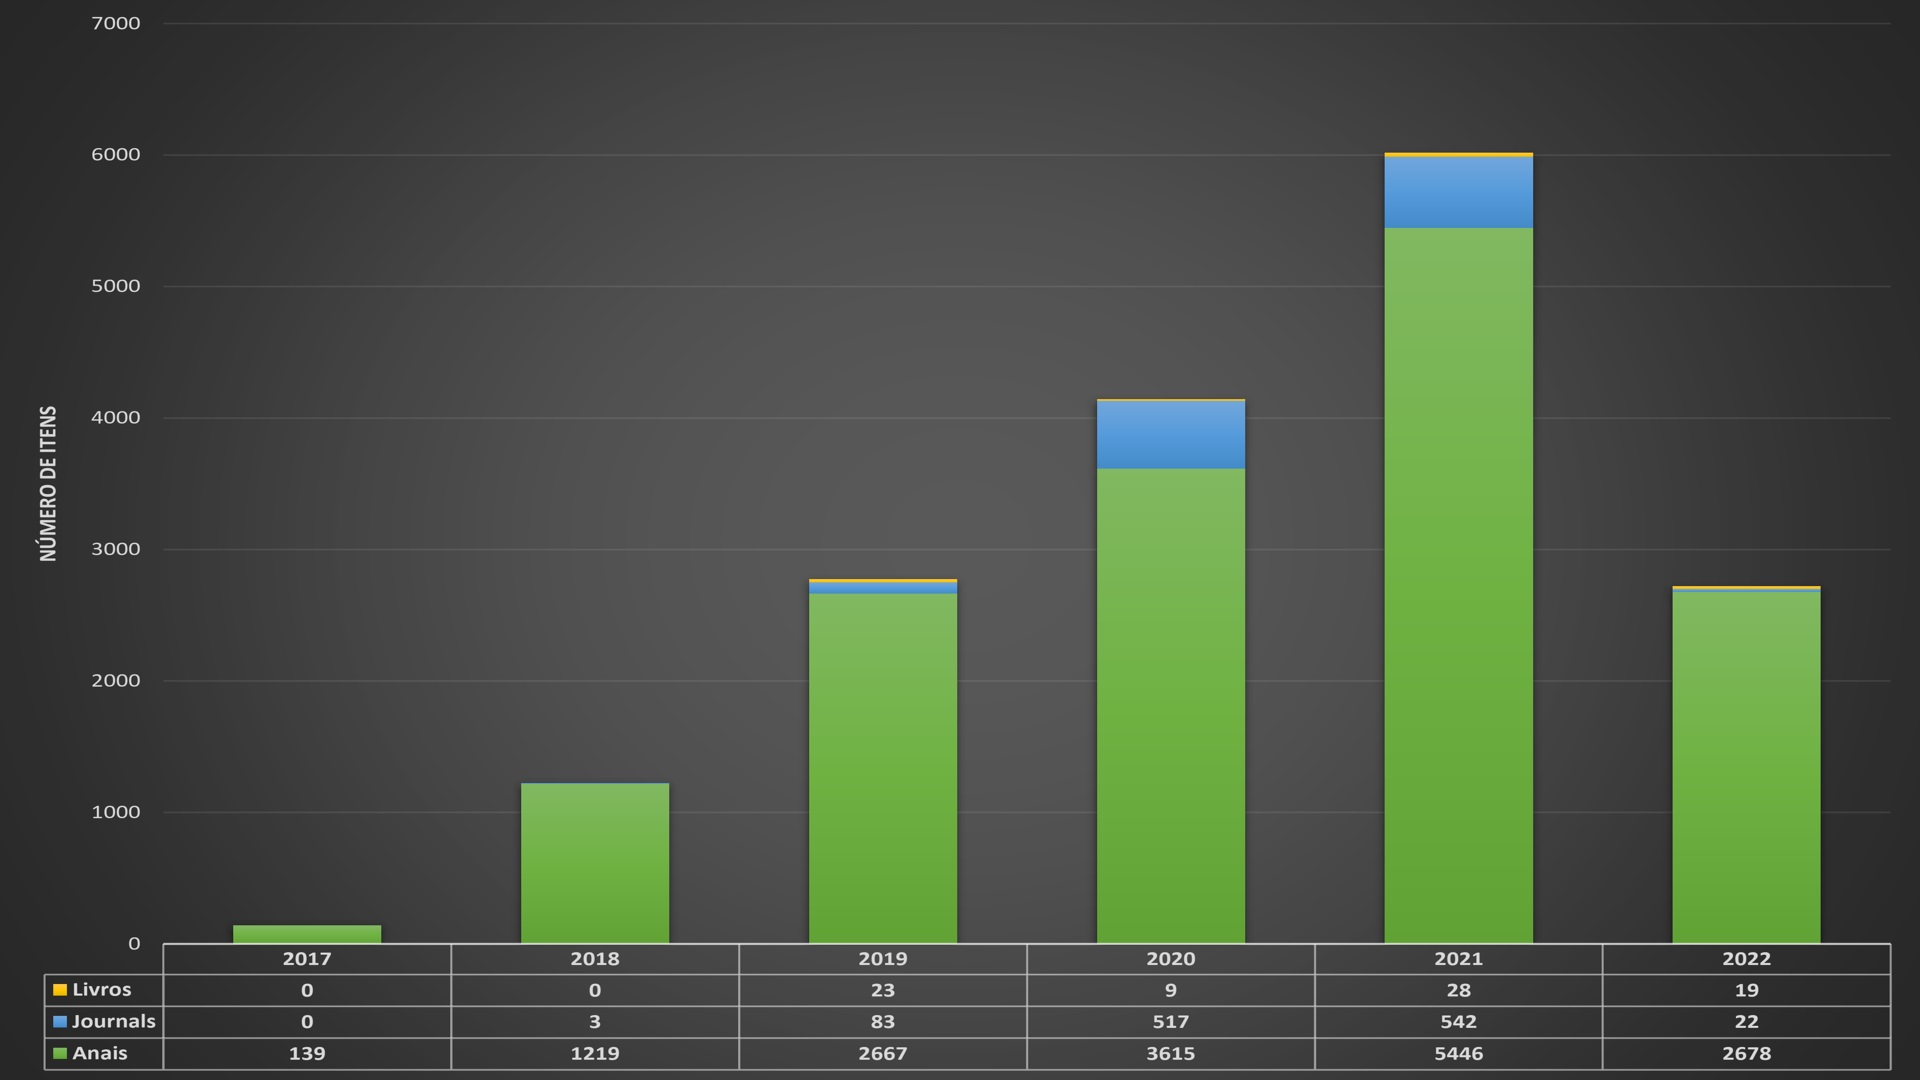
\includegraphics[width=\columnwidth]{imagens/sol.jpg}
\caption{Exemplo de legenda de figura.}\label{Fig1}
\end{center}
\end{figure}

Referência de figuras no texto \textbf{Figure \ref{Fig2}} que se expandem pelas duas colunas.

\begin{figure*}
\begin{center}
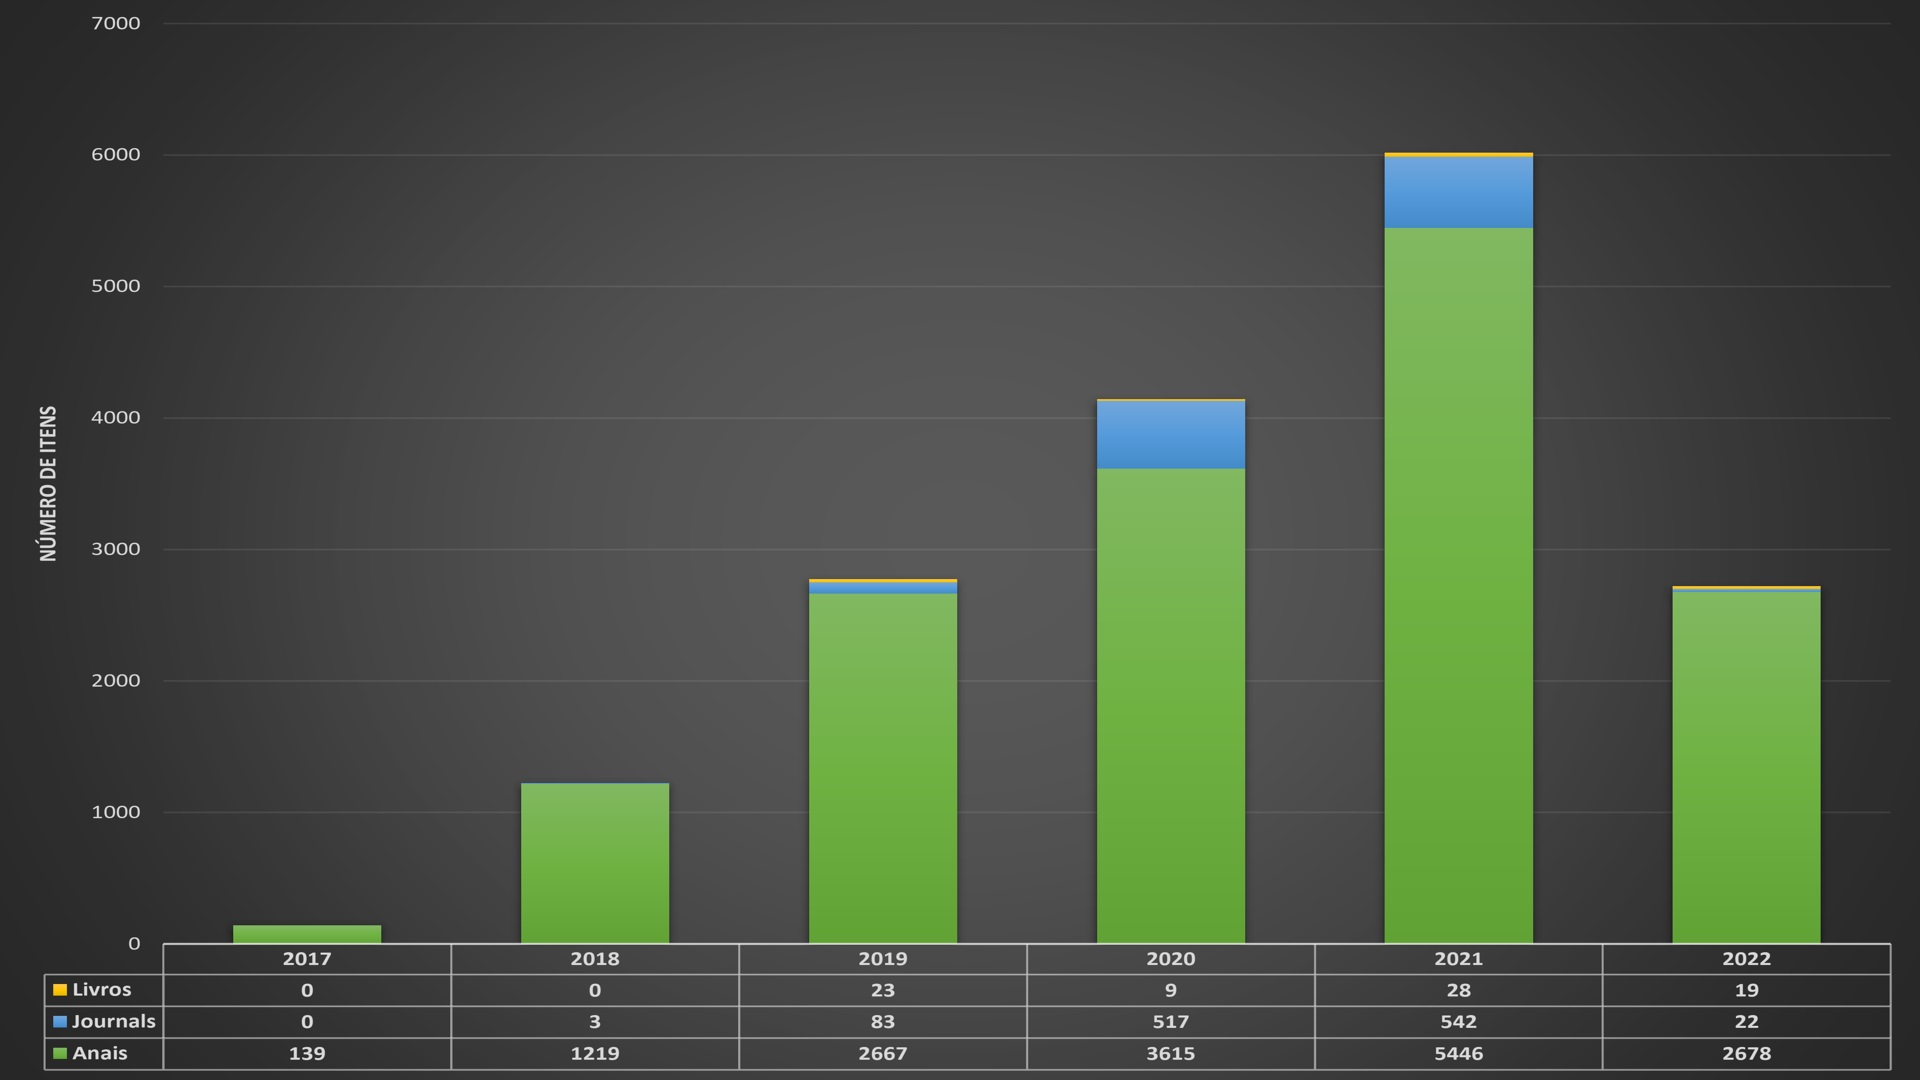
\includegraphics[width=30pc]{imagens/sol.jpg}
\caption{{Exemplo de legenda de figura.}}
 \label{Fig2}
\end{center}
\end{figure*}



\subsection{Exemplos com tabelas nativas}

\begin{table}[!ht]
\caption{Exemplo de legenda de tabela.}
\centering
\begin{tabular}{@{}cc@{}}
\hline\hline
Dimensão & Classificação\\
\hline%
 1  & 0.6232 \\
 2  & 0.9635 \\ 
 3  & 0.9724 \\ 
 4  & 0.9690 \\ 
 5  & 0.9840 \\ 
 6  & 0.9842 \\ 
 7  & 0.9873 \\ 
 8  & 0.9884 \\
 9  & 0.9873 \\ 
 10 & 0.9898 \\ 
 11 & 0.9914 \\
\hline\hline
\end{tabular}
\label{tab1}
\end{table}

Este é um texto para exemplificar como citar tabelas no decorrer do texto (ver \textbf{ Tabela~\ref{tab1}}). Como neste exemplo, é comum as tabelas aparecerem no arquivo \textit{.pdf} em um lugar distinto do que foram escritas no arquivo \texttt{.tex}. 

\subsection{Exemplo de tabelas com o pacote \texttt{tabularray}.  }


\begin{table}[!ht]
\caption{Exemplo de legenda de tabela.}
\centering
\begin{tblr}{%
columns={c},
row{even}={gray9},
row{1}={bg=gray!70, font=\bfseries}
}
\hline
Dimensão & Classificação\\
\hline%
 1  & 0.6 \\
 2  & 0.963 \\ 
 3  & 0.97 \\ 
 4  & 0.9690 \\ 
 5  & 0.9840 \\ 
 6  & 0.98423 \\ 
 7  & 0.9873 \\ 
 8  & 0.9884 \\
 9  & 0.9873 \\ 
 10 & 0.9898 \\ 
 11 & 0.991 \\
\end{tblr}
\label{tab1-1}
\end{table}


\subsection{Exemplos de citação dentro do texto}
Exemplo de citação de uma referencia (com o nome do autor antes do ano) \cite{ref3}. Outro exemplo, agora com autor e anos juntos \citep{ref4}. E mais um exemplo para a lista de referências ficar grande \citep{ref2,ref3,ref4}


\subsubsection{Equações}
\paragraph{Exemplo de Título Nível 4 (Parágrafo).}
Aqui temos um exemplo de equação no texto. Seja
\[
x=(x_1,\dots,x_n)\in R^n
\] ser um vetor \(n\)-dimensional. Aqui temos uma equação com \textit{label} para referências cruzadas.
\begin{equation}\label{eq1}
\max\limits_{x}\{x^TAx-\rho\|x\|_0:x^Tx=1\},
\end{equation}
E um exemplo de citação da Equação (\ref{eq1}). 

\paragraph{Outro Exemplo de Título Nível 4.} \lipsum[1]

\subsection{Exemplo de citação longa}
\begin{quotation}
\textit{Esta é uma citação longa. Lorem ipsum dolor sit amet, consectetur adipiscing elit, sed do eiusmod tempor incididunt ut labore et dolore magna aliqua. Lorem ipsum dolor sit amet, consectetur adipiscing elit, sed do eiusmod tempor incididunt ut labore et magna aliqua \citep{ref5}.
}\end{quotation} 



\subsection{Exemplo de tabela em duas colunas}

A Tabela \ref{tab2} é uma tabela que se expande tomando as duas colunas do documento. 

\begin{table*}
\caption{Exemplo de legenda de tabela pegando as duas colunas..} 
\centering
\begin{tabular*}{\textwidth}{@{}c\x c\x c\x c\x c\x c\x c\x c\x c\x c\x c\x c@{}}
\hline \hline
 Número   &  Vel (km/h)   & $\alpha$ (m/s$^2$)    &  $\epsilon^{(1)}$  &  $\epsilon^{(2)}$ 
         & $\delta^{(1)}$ & $\delta^{(2)}$  &  $\delta^{(3)}$    & $\gamma^{(1)}$ 
         & $\gamma^{(2)}$ & $\alpha^{(1)}$  & $\alpha^{(2)}$ \\
%
\hline
 1 & 3.5 & 2.0 & 0.20 & -0.05 & 0.00 & -0.20 & -0.05 & 0.20 & ~0.05 & 20 & 10 \\ 
 2 & 2.5 & 1.5 & 0.10 & -0.15 & 0.05 & -0.15 & ~0.00 & 0.10 & -0.05 & 20 & 40 \\ 
 3 & 3.0 & 1.8 & 0.20 & -0.05 & 0.25 & ~0.05 & ~0.20 & 0.15 & ~0.00 & 20 & 70$^a$ \\
\hline \hline
\end{tabular*}\label{tab2}
\end{table*}

